\documentclass[a4paper, 12pt]{article}

\usepackage{wrapfig}
\usepackage{graphicx}
\usepackage{mathtext}
\usepackage{amsmath}
\usepackage{siunitx} % Required for alignment
\usepackage{multirow}
\usepackage{gensymb}
\usepackage{rotating}
\sisetup{
  round-mode          = places, % Rounds numbers
  round-precision     = 2, % to 2 places
}

\usepackage[T1,T2A]{fontenc}

\usepackage[russian]{babel}

\DeclareMathOperator{\sgn}{\mathop{sgn}}
\newcommand*{\hm}[1]{#1\nobreak\discretionary{}
	{\hbox{$\mathsurround=0pt #1$}}{}}

\title{\textbf{Исследование прецессии уравновешенного гироскопа (1.2.5)}}
\author{Дудаков Семён}
\date{6 ноября 2023}

\begin{document}

	\maketitle

	\section{Введение}

	\textbf{Цель работы:} исследовать вынужденную прецессию гироскопа, установить зависимость скорости вынужденной прецессии от величины момента сил, действующий на ось гироскопа и сравнить ее со скоростью, рассчитанной по скорости прецессии.\\
	\textbf{Оборудование:} гироскоп в кардановом подвесе, секундомер, набор грузов, отдельный ротор гироскопа, цилиндр известной массы, крутильный маятник, штангенсциркуль, линейка.

	\section{Теоретические сведения}

	В этой работе исследуется зависимость скорости прецессии гироскопа от момента силы, приложенной к его оси. Для этого к оси гироскопа подвешиваются грузы. Скорость прецессии определяется по числу оборотов рычага вокруг вертикальной оси и времни, которое на это ушло, определяемоу секундомером. В процессе измерений рычаг не только поворачивается в результате прецессии гироскопа, но и опускается. Поэтому его в начале опыта следует преподнять на 5-6 градусов.  Опять надо закончить, когда рычаг опустится на такой же угол.\\
	\begin{center}$
		\begin{array}{cc}
			\includegraphics[width=0.40\textwidth]{img1.png}&
			\includegraphics[width=0.40\textwidth]{img2.png}\\
		\end{array}$
	\end{center}

	Измерение скорости прецессии гироскопа позволяет вычислить угловую скорость вращения его ротора. Расчет производится по формуле:

	\begin{equation}
		\Omega = \frac{mgl}{I_z\omega_0},
	\end{equation}

	где $m$ -- масса груза, $l$ -- расстояние от центра карданова подвеса до точки крепления груза на оси гироскопа, $I_z$ -- момент инерции гироскопа по его главной оси вращения. $\omega_0$ -- частота его вращения относительно главной оси, $\Omega$ -- частота прецессии.\\
	Момент инерции ротора относительно оси симметрии $I_0$ измеряется по крутильным колебаниям точной копии ротора, подвешиваемой вдоль оси симметрии на десткой проволоке. Период крутильных колебаний $T_0$ зависит от момента инерции $I_0$ и модуля кручения проволоки $f$:

	\begin{equation}
		T_0 = 2\pi\sqrt{\frac{I_0}{f}}.
	\end{equation}

	Чтобы исключить модуль кручения проволоки, вместо ротора гироскопа к той же проволоке подвешивают цилиндр правильной формы с известными размерами и массой, для которого легко можно вычислить момент инерции $I_\text{ц}$. Для определения момента инерции ротора гироскопа имеем:

	\begin{equation}
		I_0 = I_\text{ц}\frac{T_0^2}{T_\text{ц}^2},
		\label{moment}
	\end{equation}
	Здесь $T_\text{ц}$ -- период крутильных колебаний цилиндра.\\
    \section{Методика измерений}
	\begin{center}
		\includegraphics[width=0.8\textwidth]{img3.png}
	\end{center}

	Скорость вращения ротора гироскопа можно определить и не прибегая к исследованию прецессии. У используемых в работе гироскопов статор имеет две обмотки, необходимые для быстрой раскрутки гироскопа. В данной работе одну обмотку искользубт для раскрутки гироскопа, а вторую -- для измерения числа оборотов ротора. Ротор электромотора всегда немного намагничен. Вращаясь, он наводит во второй обмотке переменную ЭДС индукции, частота которой равна частоте врещения ротора. Частоту этой ЭДС можно, в частности, измерить по фигурам Лиссажу, получаемым на экране осциллографа, если на один вход подать исследуемую ЭДС, а на другой -- переменное напряжение с хорошо прокалиброванного генератора. При совпадении частот на эеране получаем эллипс.

    \section{Оборудование}

	Гироскоп в кардановом подвесе, секундомер, набор грузов, отдельный ротор гироскопа, цилиндр известной массы, крутильный маятник, штангенсциркуль, линейка.
    \section{Результаты измерений и обработка данных}
    
 Сначала установим параметры системы.
    \begin{align*}
     l&=(120\pm1)мм\\
     g&=(9.8155\pm0.0005)мс^{-2}\\
     \Delta m &= 1г\\
     \varepsilon_T &= 1\%
    \end{align*}
    Для измерения периода прецессии оси гироскопа выполним следующие действия. Дав ротору гироскопа раскрутиться, подвешиваем на рычаге, укрепленном на оси гироскопа, груз. Ось гироскопа приходит в движение. Следя за тем, чтобы ось гироскопа опустилась примерно на тот же угол, на который она была отклонена изначально, отмеряем целое или полуцелое число периодов (целое или полуцелое число оборотов оси гироскопа). С помощью секундомера фиксируем время, за которое было совершено это число оборотов. Период прецессии, общее время и число оборотов связанны формулой:
	
	\begin{equation}
		T = \frac{360t_{\text{полн}}}{N\varphi}
		\label{eq:period_equation}
	\end{equation}
где $t_{\text{полн}}$ -- время, за которое было совершено $N$ оборотов, $N$ -- количество оборотов, $\varphi$ -- угол смещения.
риведем данные, полученные при измерениях.

    \begin{table}[h!]
        \begin{center}
        \begin{tabular}{|l|l|l|l|l|l|}
        \hline
        $m, г$ &  $\varphi, \degree$ & $t, с$ & $\alpha, \degree$ & $\delta \alpha, \degree$ & $T, с$\\\hline
        329 &  550 &  47 & 10 & 1 & 30.8 \\ \hline
        279 &  500 &  57 & 10 & 1 & 41 \\\hline
        218 &  420 &  57 & 10 & 1 & 48.9 \\\hline
        171 &  380 &  60 & 10 & 1 & 56.8 \\\hline
        142 &  270 &  52 & 10 & 1 & 69.3 \\\hline
        116 &  240 &  54 & 10 & 1 & 81 \\\hline
        91 &  170 &  52 & 10 & 1 & 110.1 \\\hline
        77 &  130 &  48 & 10 & 1 & 133 \\\hline
        57 &  57 &  27 & 10 & 1 & 170 \\\hline
        \end{tabular}
         \caption{Измерения периода прецессии при различных массах груза}
        \end{center}

    \end{table}
    Отсюда обработав данные получаем следующие значения


    \begin{table}[h!]
        \begin{center}
        \begin{tabular}{|l|r|r|r|r|r|r|r|}
        \hline
        $№$ & $m, г$ &   $T, с$ & $\Delta T, с$ & $\Omega, с^{-1}$ & $\Delta\Omega, с^{-1}$ & $M, Нм$ & $\Delta M, Нм$\\\hline
        1 &  329 &  30.8 &    0.3 &  0.204 &  0.002 &  0.387 &  0.003 \\
        2 &  279 &  41 &    0.4 &  0.153 &  0.002 &  0.328 &  0.003 \\
        3 &  218 &  48.9 &    0.5 &  0.128 &  0.001 &  0.257 &  0.002 \\
        4 &  171 &  56.8 &    0.6 &  0.111 &  0.001 &  0.201 &  0.002 \\
        5 &  142 &  69.3 &    0.7 &  0.091 &  0.001 &  0.167 &  0.002 \\
        6 &  116 &  81 &    0.8 &  0.078 &  0.001 &  0.137 &  0.002 \\
        7 &  91 &  110.1 &    1.1 &  0.057 &  0.001 &  0.107 &  0.001 \\
        8 &  77 &  133 &    1.3 &  0.047 &  0.001 &  0.091 &  0.001 \\
        9 &  57 &  170 &    1.7 &  0.037 &  0.001 &  0.067 &  0.001 \\
        \hline
        \end{tabular}
         \caption{Обработанные данные}
        \end{center}

    \end{table}
    \paragraph{}
    В таблице выше были использованы следующие формулы

    \begin{align*}
     \Omega &= \frac{2\pi}{T}\\
     \Delta \Omega &= \Omega \frac{\Delta T}{T}\\
     M &= mgl\\
     \Delta M &= M \sqrt{\left(\frac{\Delta m}{m}\right)^2 +
                        \left(\frac{\Delta l}{l}\right)^2}
    \end{align*}
    \paragraph{}
    Теоретически есть зависимость между $\Omega$ и $M$. Выглядит оно по следующему
    \[\Omega = \frac{M}{L}\]
    где
    \[L = I_{ротор}\omega_{ротор}\]
    Построив график $\Omega(M)$ получаем значение $1/L$.
    \[\frac{1}{L}=(0.488 \pm 0.05)(Нмс)^{-1}\].
    \newpage
    \subsection{Измерение частоты вращения ротора}
    Теперь измерим момент инерции ротора для дальнейших обработок. Измерять будем крутильным маятником, предварительно "откалибровав" его цилиндром с известным моментом инерции.

    Для цилиндра имеем
    \begin{align*}
     m_{ц} &= (1616.5 \pm 0.1)г\\
     d_{ц} &= (7.78 \pm 0.01)см\\
     I_{ц} &= \frac{md^2}{8} = (1.223 \pm 0.003) 10^{-3} кгм^2\\
    \end{align*}
    \begin{table}[h!]
        \begin{center}
        \begin{tabular}{|r||r||r||r|}
        \hline
        $t_р, c$ & 31.9 & 31.85 & 31.82\\\hline
        $t_ц, c$ & 40.2 & 39.8 & 39.9\\
        \hline
        \end{tabular}
         \caption{Измерение времени за 10 периодов для цилиндра и ротора}
        \end{center}

    \end{table}
    
    Измерив периоды колебании цилиндра и ротора посчитаем момент инерции ротора
    \begin{align*}
     T_{ц} &= (4.00 \pm 0.01)с\\
     T_{р} &= (3.19 \pm 0.01)с\\
     I_{р} &= I_{ц} \frac{{T_р}^2}{{T_ц}^2} = (0.778 \pm 0.006)10^{-3} кгм^2
    \end{align*}
    Если обозначим $x=1/L$ то частота вращения ротора поучается
    \[\nu = \frac{1}{2\pi I_р x} = (419 \pm 5)Гц\]

    При измерении этой частоты осцилографом с помощью фигур лиссажу получаем значение
    \[\nu_{осц}=(380 \pm 1)Гц\]
    \subsection{Измерение момента трения}
    Во время эксперимерта ось гироскопа опускалось в первую очередь из за трения в вертикальной оси. Для оценивания момента сил трения можно воспользоватся данными про угол наклона $\alpha$ за время эксперимента $t$. Формула момента трения приобретает следующий вид.
    \[M_{тр} \approx \frac{L\alpha}{t}\]
    Для наших данных получаем следующие значения.


    \begin{table}[h!]
        \begin{center}
        \begin{tabular}{|l|r|r|r|r|r|r|r|r|r|r|}
        \hline
        $M_{тр}, 10^{-4}Нм$ &  9.0 &  8.0 &  8.0 &  8.0 &  9.0 &  7.0 &  8.0 &  8.0 &  9.0 &  8.0 \\\hline
        $\Delta M_{тр}, 10^{-4}Нм$ &  1.0 &  1.0 &  1.0 &  1.0 &  1.0 &  1.0 &  1.0 &  1.0 &  1.0 &  1.0 \\
        \hline
        \end{tabular}
         \caption{Моменты сил трения}
        \end{center}

    \end{table}
    Усредняя получаем
    \[M_{тр}=(8.2 \pm 1.2) 10^{-4}Нм\]
    \section{Обсуждение результатов}
    \begin{itemize}
			\item Была определена теоретически и экспериментально угловая скорость регулярной прецессии гироскопа. Полученная точность теоретически определенной величины совпадает с точностью, с которой можно определить момент инерции ротора гироскопа, так как эта величина вносит наибольший вклад в погрешность. 
			\item Был определен момент инерции ротора гироскопа: $I_{0} = \left( 7,78 \pm 0,06 \right) \cdot 10^{-4}\quad \text{Кг} \cdot \text{м}^{2}$; Основной вклад -- погрешность измерения радиуса цилиндра, с помощью которого определялась данная величина.
            \item Был определен момент сил трения, возникающих в оси карданного подвеса: $M = (8,2 \pm 1,2)\cdot 10^{-4}\quad \text{Н}\cdot\text{м}$;  Основной вклад: погрешность измерения угла отклонения оси от горизонтальной плоскости, погрешность фиксирования прохождения оси через начальную точку.
   \end{itemize}
    \section{Заключение}
    Как видим частоты вращения близки, но в пределах погрешности они не совпадают. В чем причина расхождения? Пытатся объяснить тем, что мы не учитываем косинус угла при подсчете момента, или тем что угловая скорость прецессии в этом виновата не получится, слишком мелкие поправки. По моему мнению проблема состоит в измерении момента инерции ротора, так как при неуравновешенных колебаниях момент инерции искажается.
    \newpage
    \begin{sidewaysfigure}
        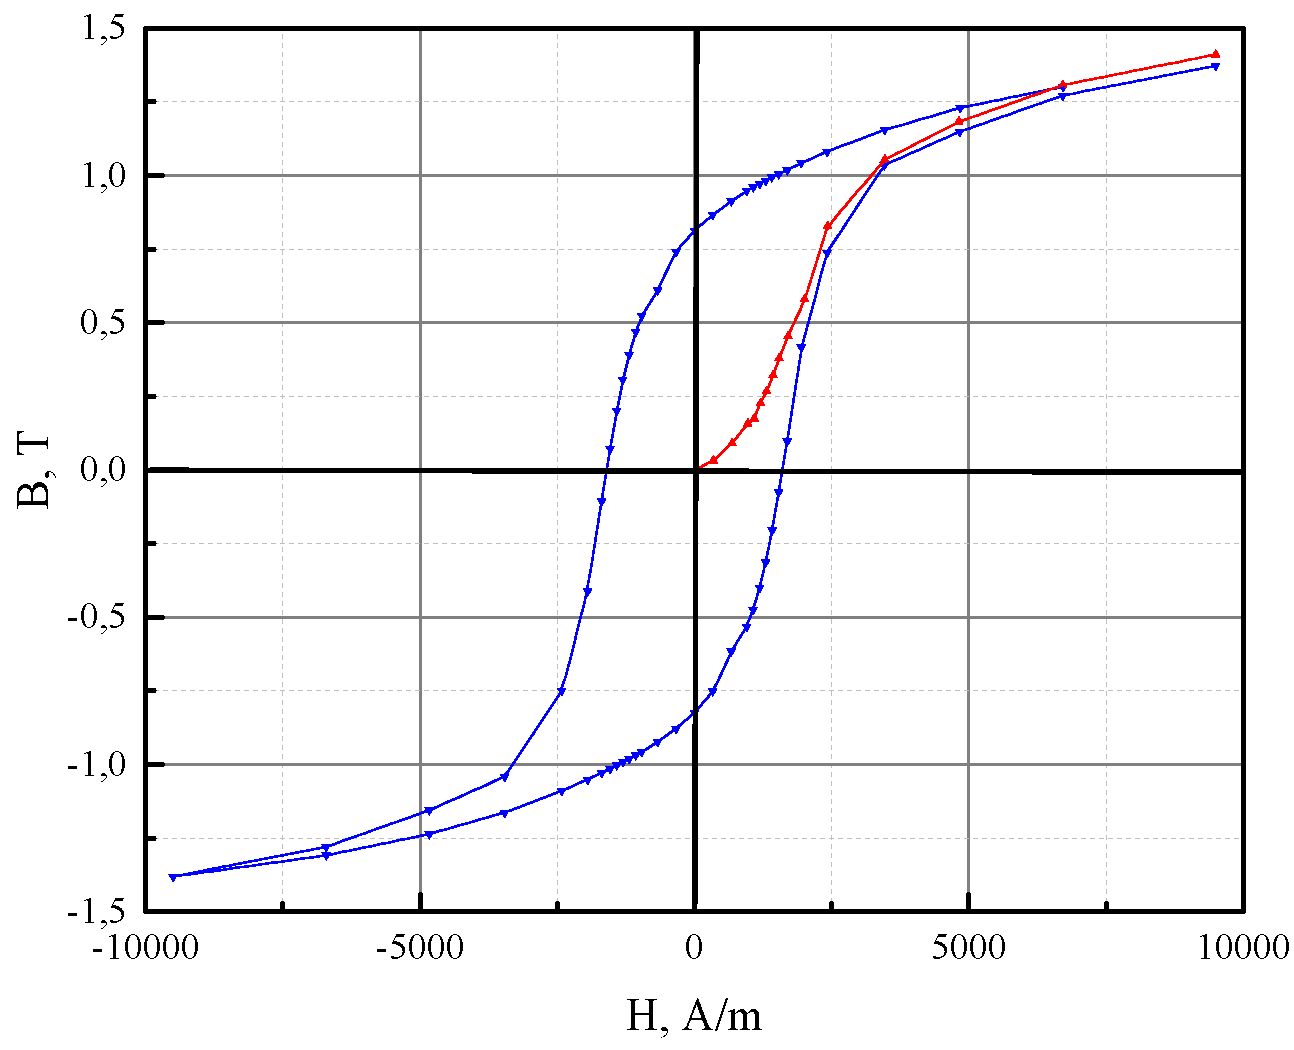
\includegraphics[width=1.20\textwidth]{plot.png}
        \caption{График $\Omega(M)$}
    \end{sidewaysfigure}



\end{document}